\section{Discussion}
\label{s:discussion}

In this part, we will discuss two kinds of deployment of simhash based cloaking detection system: server-based and crowdsoucing.

\subsection{Server-based cloaking detetion system}
In server-based cloaking detection system,
we first collect targeted search terms includes commecial terms, cloaking oriented terms and hot trend words.
Using these search terms, the cralwer extracts the search results from the search engines for seven times.
In six times, the crawler disguises as Google crawler by using the Google Agent and crawl data. With this data that
is crawled from Google view, the system uses the simhash method to model the websites. The last
time, the crawler disguises as normal user by using user agent. The system compares simhash value from user view and
website model learned from Google view. From the comparsion result, the system judges if the website is cloaking
or not. 
Server based cloaking detection system has pros and cons. The deployment of server based cloaking dectetion system
is pratical and could be deployed
easily. The tradeoff of easy deployment is inefficient in IP cloaking detection. Usually, the servers IP addresses
are in a range,  scammers could find this range and serve benign content to crawlers. One solution is buying numerous IP addresses
from ISP providers and distributing IP addresses as users distribution. This increases cloaking detection cost. In
addition, distributing IP addresses as users distribution is hard. Further, server-based cloaking detection system is infeasiable
to detect cloaking in search engine marketing(SEM). As we mentioned, using the crawlers to visit websites in SEM field
increases the advertisement cost of websites. Moreover, different websites has different changing periods. For example, Yahoo website
updates very quickly. Apple website updates slowly. Finding different crawling periods for different websites is difficult. 

\subsection{Crowdsourcing}
Crowdsourcing cloaking detection system includes user-side and server-side component. In user side, users needs to install the cloaking
detection extension in their browers. While users click search results and view websites, the extention calculate the simhash value based on 
website content and layouts. After calculation, extension packs URL and simhash value and sends to server. Server passively receives (URL, simhash value)
pairs from users. Server also utilizes crawlers to extract content several times in this URL from search engine view (crawler uses Google bot agents).
Server uses these extract content to model the website. From the comparison result between (URL, simhash value) from users and website model,
server could decide if the website is cloaking or not. From previous study, cloaking includes phishing and malware downloading. Based on cloaking
detection result, server categorizes cloaking and update blacklists in browsers' extensions. Updating blacklists and warning users phishing and
malware downloading is users incentive to install our extension.

Previously, we describe our crowdsoucing workflow. Next, We discuss the pros and cons for this approach. The first advantage is privacy. Instead of solicting
website content from users, the system solicited a 64 bits simhash value from users. From this 64 bits value, system couldn't do reverse engineering to
get original content. In addition, the system could intergrate with RAPPOR~\cite{erlingsson2014rappor}, which protect the privacy of URL.
Because the workflow is similar to safe browsing API ~\cite{rajab2013camp} , we argue that this can be easily
extended in current framework, the only different is that (URL, simhash value)
pair is processed through RAPPOR to achieve anonymity.

In addition, the crowdsouring deployment introduces low traffic. Browsers only send a 64 bits value for
each URL. This won't jam traffic. Further, the crowdsoucing deployment wouldn't affect the model of SEM. Each click on advertisements of search engines is
from real users instead of crawlers. Advertisers don't need to pay extra money for cloaking detection. 


Employ RAPPOR~\cite{erlingsson2014rappor} to provide user privacy gurantee.

pros: 	1.privacy 2.Low traffic. 3.SEM 4.Distributed computation 
5. Remove the need to do redirect cloaking detection, leveraging the feature
that the end goal of attackers is to reach user
6. could decide crawl period passively based on user clicks, data received are
based on real user’s clicks, say, website traffic
%
%cons: user incentives. 
%Solution: Plugin to detect suspicious websites. API


\begin{figure}[t]
  \centering
  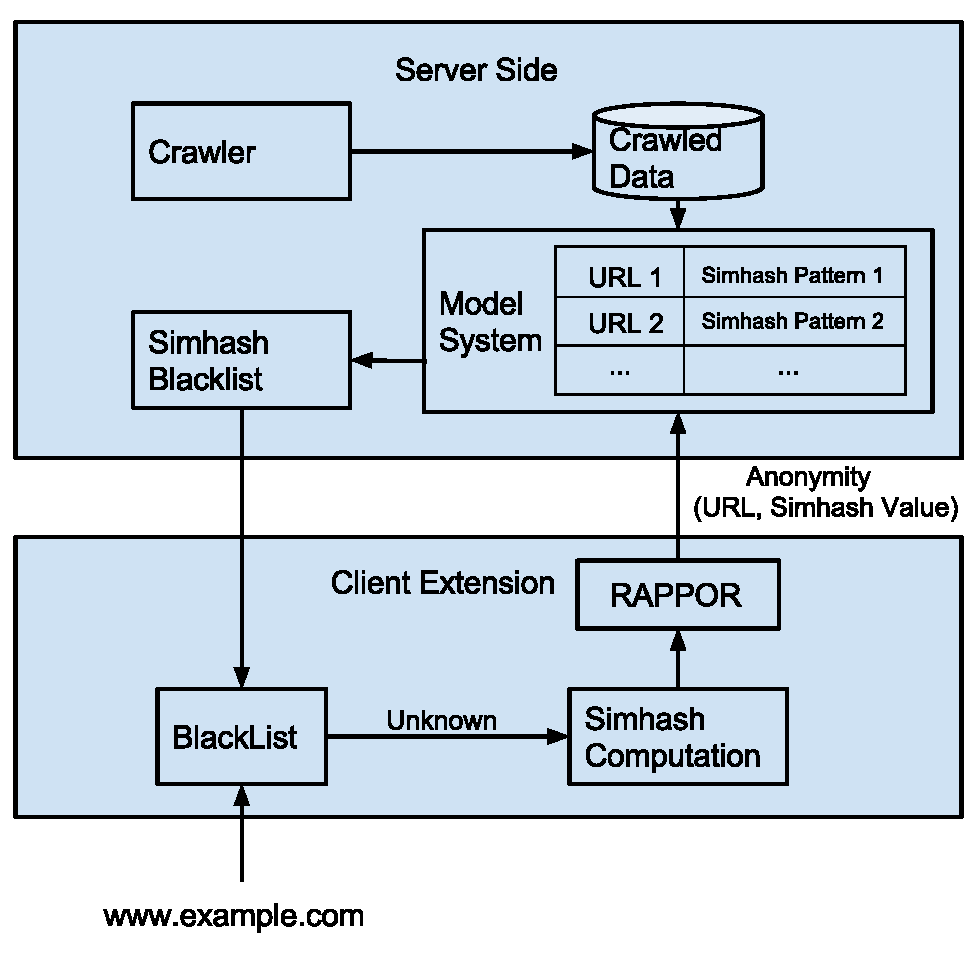
\includegraphics[width=.45\textwidth]{fig/crowdsourcing-cloaking-detection-system}
  \caption{Workflow of crowdsource cloaking detection sysetem}
  \label{fig:workflow}
\end{figure}


The workflow ~\autoref{fig:workflow} is to collect page contents simhash on the user side, and compare
them to simhash of the same link from ad serving company to find cloaking. When
the differences of the simhashes are significantly large, the page is marked
cloaking. We generate two simhash for page content and structure respectively.
Intuition behind this is, simhash difference between different sites are larger
than different visits of the same site. We build a two-phase system to detect
cloaking: cluster learning phase, and cloaking detection phase. In the cluster
learning phase, an ad company visit urls and generate simhash from its content
with its owned IP, and learn pattern and distribution of the simhashes, i.e.
simhash-based website model. In the cloaking detection phase, the ad company
collects simhash from its users. Compare them with learned patterns, return
cloaking score or mismatch

